% !TeX root = ../../main.tex

\section{Economic scenarios}

\begin{table}[H]
\centering
\caption{Percentage change in parameters for scenario analysis}
\label{tab:scenario_analysis}
\begin{tabular}{@{}l|llll@{}}
\toprule
                      & \multicolumn{4}{c}{\textbf{Scenarios}}                                                        \\
\textbf{Parameter}    & \textit{\textbf{Best case}} & \textit{\textbf{Base case}} & \textit{\textbf{Worst case}} & \textit{\textbf{COVID case}} \\ \midrule
WACC                  & -\SI{30}{\percent}                       & -                          & \SI{30}{\percent}                         & -                            \\
CAPEX                 & -\SI{30}{\percent}                       & -                          & \SI{30}{\percent}                         & -                            \\
Price of product      & \SI{30}{\percent}                        & -                          & -\SI{30}{\percent}                        & -                            \\
Production delay      & No delay                    & No delay                   & 3 year delay                 & 3 year delay                 \\
Operational days      & -                           & -                          & -                            & -\SI{40}{\percent}                        \\
Cost of raw materials & -                           & -                          & -                            & -\SI{40}{\percent}                        \\
Interest rate         & -                           & -                          & -                            & -\SI{40}{\percent}                        \\\bottomrule
\end{tabular}
\end{table}

\begin{wrapfigure}{r}{8cm}
    \vspace{-0.9cm}
    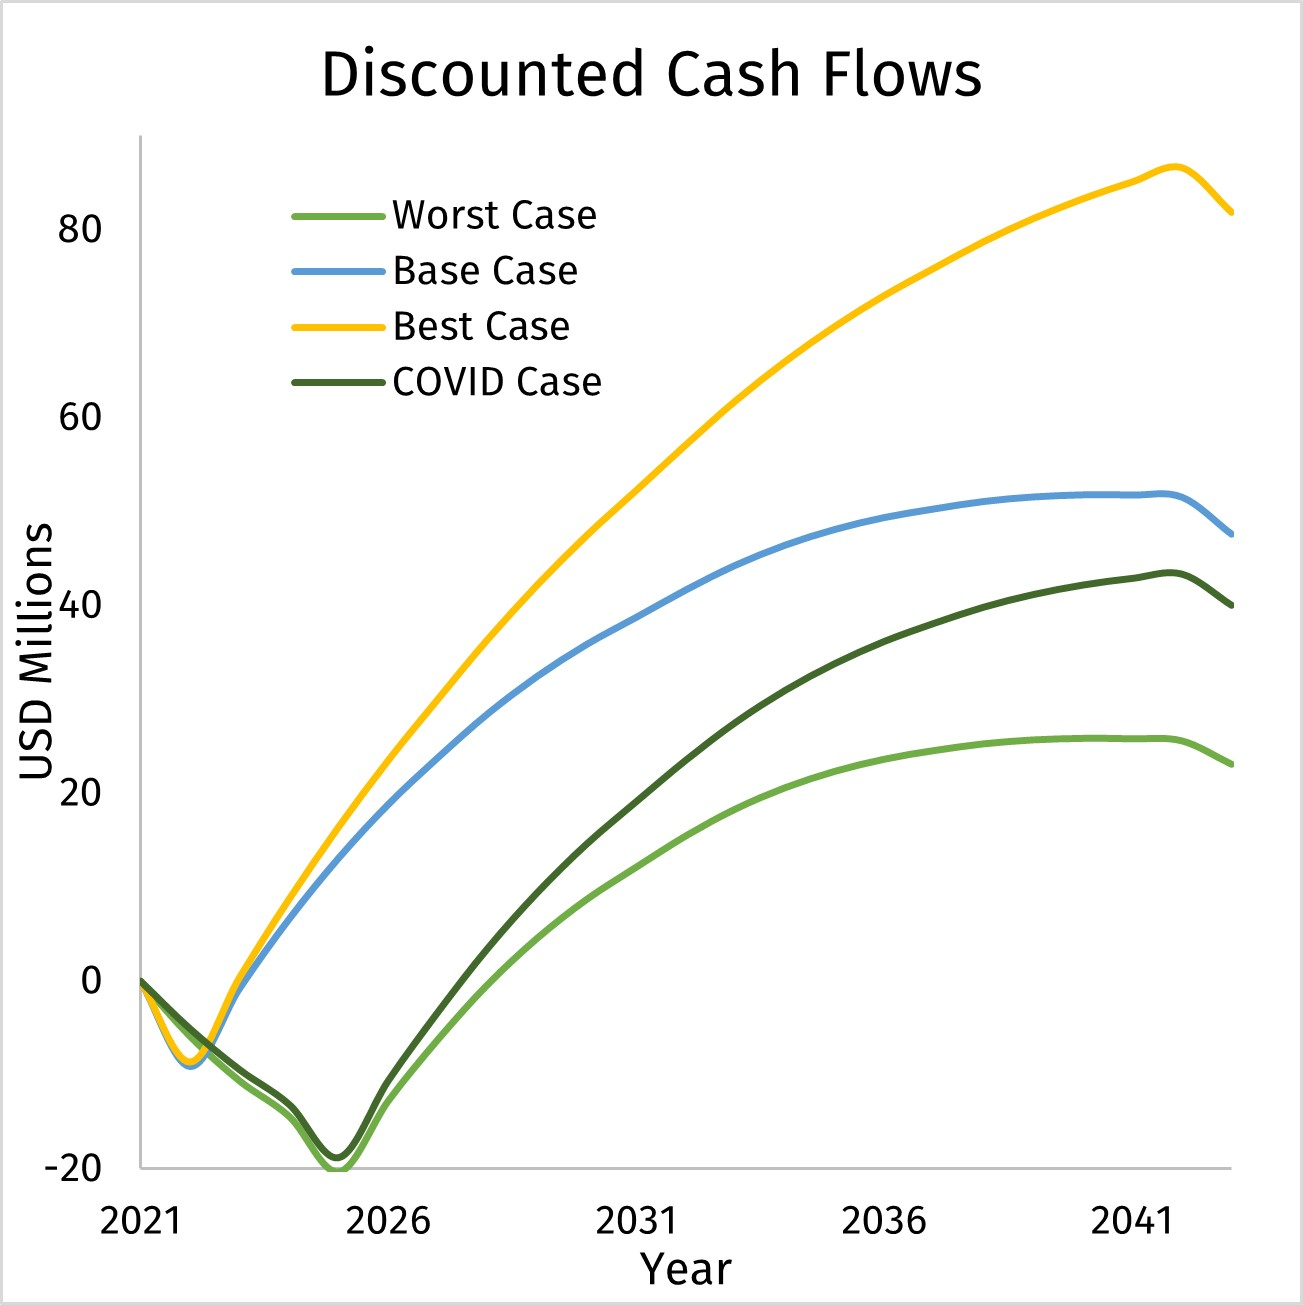
\includegraphics[width=0.47\textwidth]{chapters/6-economics/figures/DCF.jpg}
    \caption{Discounted cash flow profile for different scenarios}
    \label{DCF_scenario}
\end{wrapfigure}

Four scenarios were analysed to understand the combined effect of the parameters tested in Section \ref{sec:sensitivities-kpis}. Table \ref{tab:scenario_analysis} summarises the fluctuations made in each scenario. The best- and worst-case scenarios were based off the most extreme variations of each parameter in the sensitivity analysis. 

One scenario was related to a situation where COVID-19 resurfaced in Nanjing, China, and restriction measures were in place till 2026. The number of operational days per year was expected to drop by \SI{40}{\percent} based on the lockdown period during the initial outbreak of coronavirus in 2020 (bbc 20). A \SI{40}{\percent} decrease in the cost of raw materials was also modelled into the scenario, based on the fall in toluene prices between January and April 2020 (sunsirs 21). Similarly, a \SI{40}{\percent} decrease in interest rate was applied, based off the drop in the average Chinese interest rate between January and April 2020 (statista 21). A 3-year delay in production was also anticipated due to reduced labour availability. The price of Nitroma’s products was not expected to change considerably, as discussed in Section \ref{sec:market-analysis}. It should be noted that the coronavirus conditions were only applied until 2026, after which the base case conditions were restored in the scenario test.

Figure \ref{DCF_scenario} shows Nitroma’s discounted cash flows till 2043 for each tested scenario. Across all the tested scenarios, the minimum ending cash balance was \$23.1 million and the longest payback period was 10.3 years. These results show the robustness of this project and should enhance the confidence of the shareholders.
